\chapter{Data processing with \ctapipe{}}
\label{ch:data-processing}

The analysis in this work was done with the open-source low-level data processing software for \cta{},
\ctapipe{} \cite{ctapipe}, more specifically, version \texttt{0.15.1}.
% The version used is the development version \texttt{0.15.1.dev166+gf26107f},
% henceforth shortened to version \texttt{0.15.1}.
The goal of \ctapipe{} is to provide a complete analysis
framework ranging from data calibration and image extraction to the reconstruction of events and the
analysis of their properties. In this chapter, I will first describe how the data
were simulated in \autoref{sec:data-simulation} and then, in \autoref{sec:data-levels}, explain the different
data levels and \ctapipe{}'s various analysis steps. In \autoref{sec:pipeline} I will
explain the full pipeline created for this work.


\section{Data simulation}
\label{sec:data-simulation}

In its current in-development state, \ctapipe{} is used and tested with simulated data, as the software
can only be sufficiently tested when the output is compared to truth data. This data is created with the help of
\gls{mc} simulations. The software used for these simulations is called \gls{corsika} \cite{corsika} and
allows for detailed simulation of \glspl{eas} initiated by \glspl{hecr}. The showers are observed by
a virtual \gls{iact} array, the \texttt{sim\_telarray} \cite{bernlohr2008}, that allows simulating the optics
of various mirror and camera geometries via ray-tracing of incoming photons. This also includes
simulations of imperfections or misalignments of the mirrors of each telescope. The resulting so-called
\texttt{simtel} data is used in \ctapipe{} and can be processed as described in \autoref{sec:data-levels}
and \autoref{fig:ctapipe}. Some of the data properties are listed in \autoref{tab:simtel}.

This data is the basis for the analysis in this work. A total of around \(\num{27}\)\,k telescope events
(\sim\(\num{12}\)\,k array events) throughout \(\num{20}\) \texttt{simtel} runs of diffuse gamma data
were used for the initial analysis, \ie the testing of different parameters as described in
\autoref{sec:hyperparameters}. After processing the individual runs and merging them into one large
file, this file is being processed for the aforementioned parameters. %  \(\num{27353}\) \(\num{12668}\)

Once promising parameters are found, a larger dataset, containing around \(\num{1.3}\)\,M telescope events
(\sim\(\num{620}\)\,k array events) throughout \(987\) runs, is processed with these
selected settings, allowing for more statistics and a better comparison of the cleaning algorithms.
%\(\num{1331328}\) \(\num{621848}\)
\begin{table}
    \centering
    \caption{Simtel data properties of the \gls{corsika} simulation used for the datasets in this works
    analysis.}
    \label{tab:simtel}
    \rowcolors{0}{white!92!black}{}
    \begin{tabular}{l r}
        \hiderowcolors
        & Diffuse Gamma data \\
        \showrowcolors
        {Energy range / \si{\tera\eV}} & \numrange[range-phrase={--}]{0.003}{330} \\
        {Zenith angle / \si{\degree}} & \num{20} \\
        {View cone angle / \si{\degree}} & \num{10} \\
        {Number of showers} & \num{50000} \\
        {Spectral index} & \num{-2.0} \\
        {Maximum scatter range / \si{\meter}} & \num{1900} \\
    \end{tabular}
\end{table}


\section{Data Levels in \ctapipe{}}
\label{sec:data-levels}

There are several data levels in \ctapipe{}, spanning from the raw data \rzero{} to the reconstructed events
\dlt{}, with the raw data levels being denoted by an \textbf{R} and the calibrated data levels by a \textbf{D}.
\autoref{fig:ctapipe} shows a simplified overview of the data levels and the analysis steps.
The raw data level \rzero{} is the data that comes directly from the photodetectors. The time-resolved
signal of the data is calibrated from \rzero{} to \rone{}. The data volume gets reduced
(\rone{} \rightarrow \dlz{}) by detecting waveform peaks for each pixel and then integrating them.
\begin{figure}
    \centering
    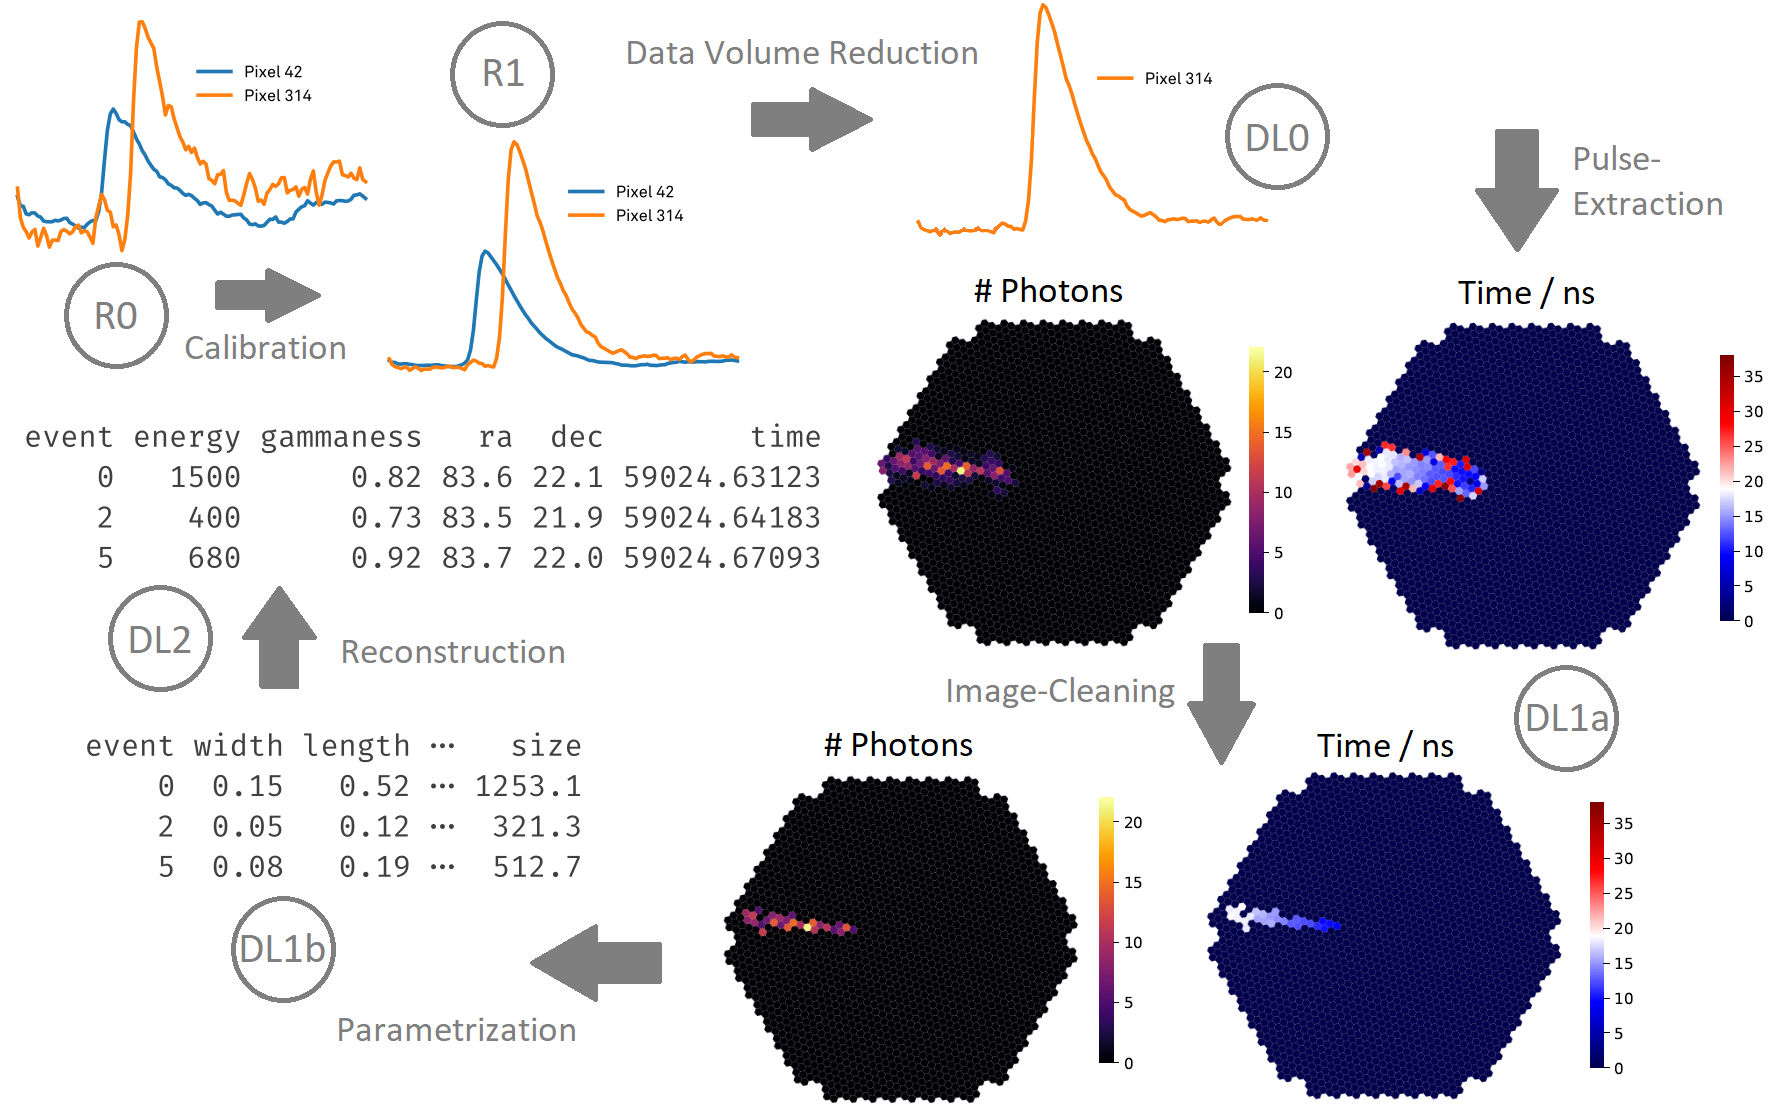
\includegraphics[width=\textwidth]{graphics/ctapipe.png}
    \caption{Data levels in \ctapipe{}. Raw data levels are denoted by an \textbf{R} and calibrated
    data levels by a \textbf{D}. The raw data first gets calibrated (\rzero{} \rightarrow \rone{})
    and then reduced in volume by selecting waveforms (\rone{} \rightarrow \dlz{}). From there the
    images are extracted (\dlz{} \rightarrow \dloa{}) and cleaned with a cleaning algorithm. This
    allows for parametrization of the events (\dloa{} \rightarrow \dlob{}). The parametrized events
    can then be reconstructed (\dlob{} \rightarrow \dlt{}) \cite{noethe_thesis, hackfeld}.}
    \label{fig:ctapipe}
\end{figure}

The \dlz{} data level is the first level being stored and also the first level to be processed from
the simulation datasets used in this work. From \dlz{} to \dloa{}, the photon images are extracted
by integrating the waveform peaks of each pixel, whilst the time ("peak times", compare \autoref{fig:ctapipe})
are extracted by finding the rising edge of the pulse. The resulting images are cleaned by cleaning algorithms,
which, in turn, allows for a parametrization of the events from \dloa{} to \dlob{}.
% From \dlz{} to \dloa{}, the images of the data are extracted
% from the time pulses, which are then cleaned by a cleaning algorithm, allowing for parametrization
% of the events (\dloa{} \rightarrow \dlob{}).
The cleaning is a necessary step, especially for
low-energy events, where the actual signal is harder to distinguish from the \gls{nsb}. The cleaning algorithms
of \ctapipe{} are introduced in \autoref{sec:cleaning-algorithms} and can be roughly categorized into
time-based and non-time-based algorithms.

While the latter are selecting pixels based on charge thresholds which
subsequently might lead to the need for a higher threshold, the former also takes the arrival times of
pixels in the camera frame into account, allowing for a lower charge threshold.

The advantage of a lower charge threshold allows the selection of more of the signal at lower energies.
Once the events are cleaned and parametrized, they can then be reconstructed (\dlob{} \rightarrow \dlt{})
and stored on the \dlt{} data level, which consists of an event list with reconstructed gammaness---a value
that predicates how likely an event was produced by a gamma---, direction and energy.


\section{This work's data processing pipeline}
\label{sec:pipeline}
In this work, the data processing pipeline is as follows: First, several simulation data runs are
selected and processed with \ctapipe{}. Then, the datasets are merged and serve as a basis for a re-run
of the combined dataset with various parameter combinations described in \autoref{ch:finding-hyperparams}.

The settings for \ctapipe{} are saved in two configuration files: First, a file, that sets up the
cleaning process and what data to write to the output file. For the preprocessing step of this work's
pipeline, the cleaning settings are not relevant, as this step only serves to create a merged dataset.
The second file contains a list of all the allowed telescope IDs. This allows a selection of the telescopes
that are used in the analysis. This is especially helpful if one wants to only analyze \gls{mst}-related
data, like in this work.

For the re-run of the combined dataset, the cleaning settings are used\footnote{As opposed to the preprocessing step},
however, since this step is the heart of this work's search for the optimal hyperparameters.
The configuration files used are shown in \hyperref[ap:config_files]{appendix \ref{ap:config_files}}.

Each resulting dataset can then be processed on an array or telescope data level, resulting in
\dloa{} image plots, values for the angular resolution and the efficiency as well as metrics for the
performance. An in-detail description of how this helps to compare the performance of the different
cleaning algorithms can be found in \autoref{sec:hyperparameters}. A schematic overview of the data
processing pipeline of this work is shown in \autoref{fig:data-processing}.

\begin{figure}
    \centering
    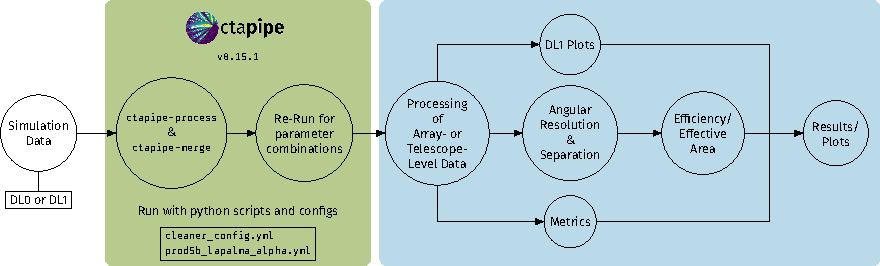
\includegraphics[width=\textwidth]{graphics/data_pipeline.pdf}
    \caption{Schematic overview of the data pipeline used for this work. Single runs of the simulation
    data are processed with \ctapipe\texttt{-process} and then merged via the tool \ctapipe\texttt{-merge} (green shaded area).
    The merged data is then processed on the array or telescope data level resulting in scores for metrics
    as well as \dlo{} \texttt{images} and plots for the angular resolution and the effective area (blue shaded area).}
    \label{fig:data-processing}
\end{figure}


